\section{Les composants clés du cloud computing :}
Pour comprendre le fonctionnement du Cloud, il faut connaitre ses deux composants essentiels, à savoir la notion de Virtualisation et de Data center.

\subsection{Virtualisation :}
C'est l'ensemble des techniques matérielles et/ou logiciels qui permettent de faire fonctionner sur une seule machine, plusieurs systèmes d'exploitation (appelées machines virtuelles (VM), ou encore OS invité).

Même s'il existe plusieurs types de virtualisation, la forme la plus populaire de virtualisation dans le cloud est la virtualisation des serveurs qui consiste à dématérialiser le comportement et les données d'un serveur ou d'une machine, de façon à faire tourner plusieurs de ces instances dématérialisées sur un même serveur physique.

De cette façon, les diffiérentes instances créées se partagent les ressources du serveur physique. Cela permet une plus grande modularité dans la répartition des charges, une facilité dans l'administration des serveurs et une réduction des coûts.

\begin{figure}[h]
	\centering
	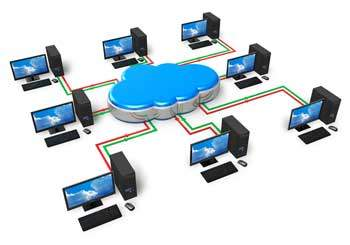
\includegraphics[scale=0.8]{img/2.1}
	\caption{La Virtualisation}
\end{figure}

\subsection{Les Data Center :}
Un data center ou centre de données, c'est un site physique qui a une infrastructure composée d'un réseau d'ordinateurs et d'espaces de stockage, Il peut être interne ou externe à l'entreprise. Ces sites sont des salles remplies de baies de stockage, utilisées par de nombreuses entreprises et autres organisations gouvernementales

\begin{itemize}
\item  \textbf{Les composants du Data Center :} Un centre de données basique regroupe des serveurs, des sous-systèmes de stockage, des commutateurs de réseau, des routeurs, des firewalls, et bien entendu des câbles et des racks physiques permettant d'organiser et d'interconnecter tout cet équipement informatique.
\begin{figure}[h]
	\centering
	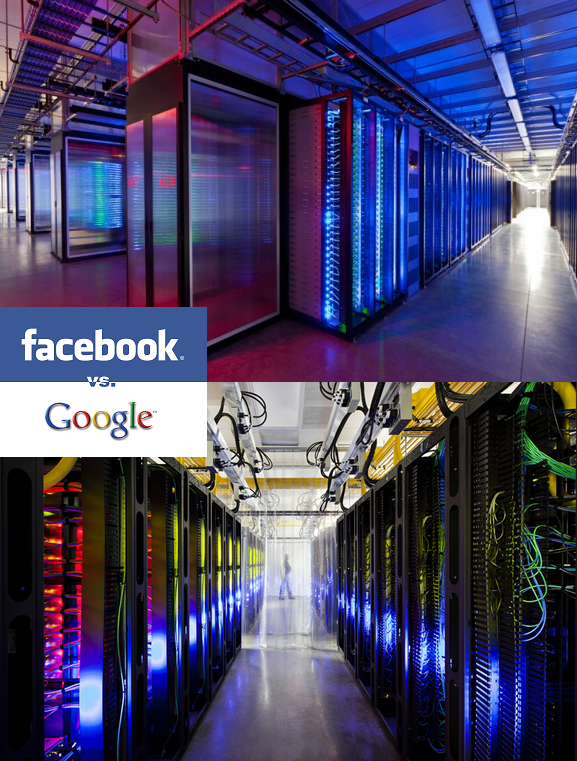
\includegraphics[scale=0.4]{img/2.2}
	\caption{Exemple de data center (ceux de Facebook et Google)}
\end{figure}
\bigskip \bigskip \bigskip \bigskip
\item  \textbf{L'architecture du data center :} Théoriquement, n'importe quel espace suffisamment vaste peut servir de Data Center. Cependant, le design et l'implémentation d'un data center nécessite de prendre plusieurs précautions. Par-delà les problèmes basiques du coût et des taxes, les sites sont sélectionnés sur de nombreux critères, comme la localisation géographique, la stabilité météorologique, l'accès aux routes et aux aéroports, la disponibilité énergétique, les télécommunications ou encore l'environnement politique.

Pour fonctionner correctement, un Data Center doit aussi abriter l'infrastructure adéquate : un système distribution d'énergie, un commutateur électriques, des réserves d'énergie, des générateurs dédiés au backup, un système de ventilation et de refroidissement, et une puissante connexion internet. Une telle infrastructure nécessite un espace physique suffisamment vaste et sécurisé pour contenir tout cet équipement.
\end{itemize}
\begin{figure}[h]
	\centering
	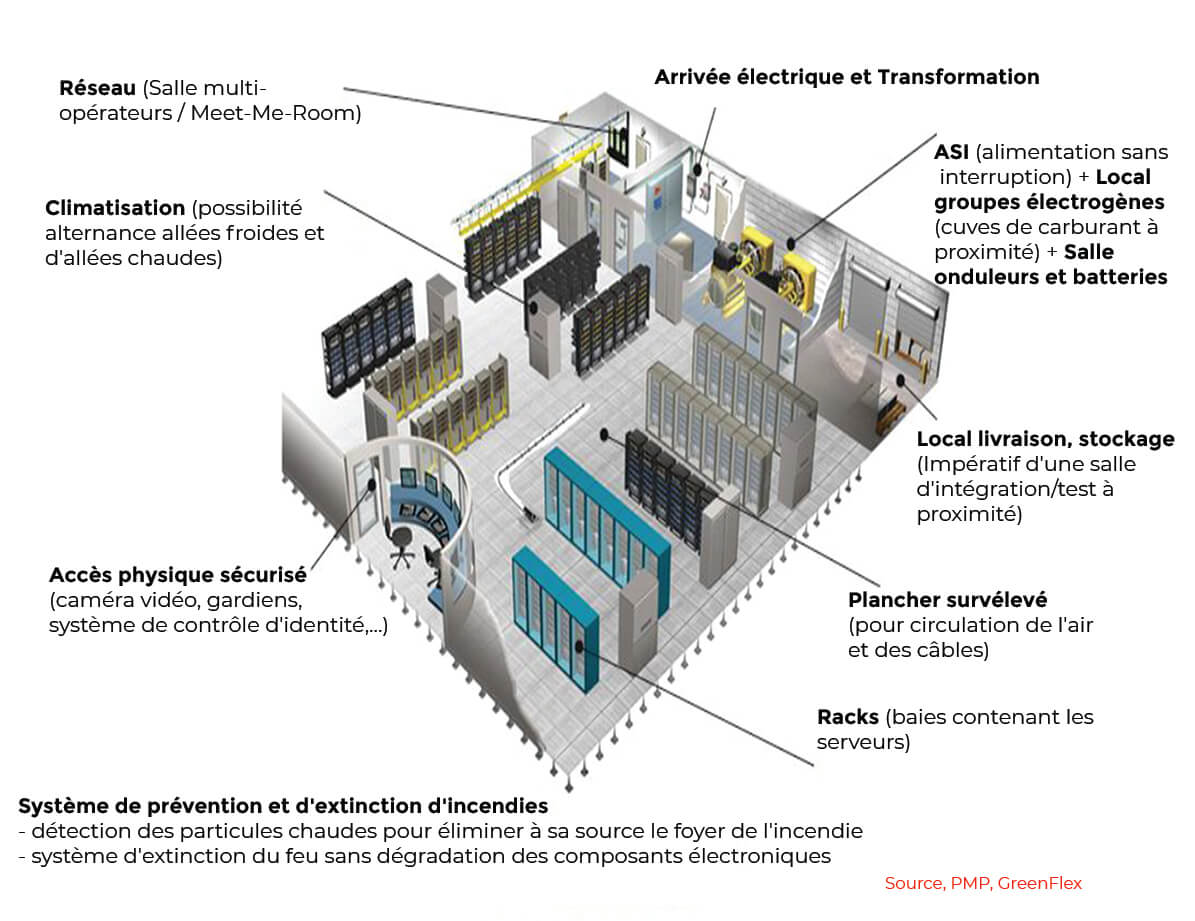
\includegraphics[scale=0.2]{img/2.3}
	\caption{Architecture du data center}
\end{figure}




